
\section{Experiment}
\subsection{Phase 1 - Training}

Each network was trained ten times over the course of multiple hours resulting in a representatively distributed set of trained networks.
Figure \ref{fig:training_times} visualizes the relations between the average training times.

\begin{figure}[hbt]
    \centering
    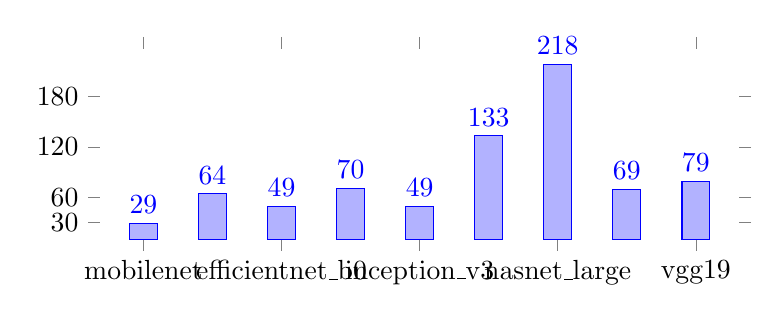
\begin{tikzpicture}
      \begin{axis}[ybar,
            width=100mm, height=40mm,
            x axis line style = { opacity = 0 },
            symbolic x coords = {mobilenet, nasnet\_mobile, efficientnet\_b0, xception, inception\_v3, efficientnet\_b5, nasnet\_large, vgg16, vgg19},
            ytick={30,60,120,180,240},
            nodes near coords,
        ]
        \addplot coordinates { 
            (mobilenet,         29)
            (nasnet\_mobile,    64)
            (efficientnet\_b0,  49)
            (xception,          70)
            (inception\_v3,     49)
            (efficientnet\_b5, 133)
            (nasnet\_large,    218)
            (vgg16,             69)
            (vgg19,             79)
        };
      \end{axis}
    \end{tikzpicture}
    
    \caption{Figure: Average Training Time in seconds}
    \label{img:avg-train-time}
\end{figure}




No direct corellation between parameter count and training time can be determined.
NasNet Large takes by far the longest to train with an average of approximately 3.5 minutes. 
MobileNet was the fastest to train with slightly under 30 seconds.


\begin{figure}[h!]
    \centering

    \begin{figure}[h!]
    \centering

    \begin{figure}[h!]
    \centering

    \input{fig/graph/validation_accuracies.tex}

    \caption{Validation Accuracies}
    \label{fig:validation-accuracies}
\end{figure}

    \caption{Validation Accuracies}
    \label{fig:validation-accuracies}
\end{figure}

    \caption{Validation Accuracies}
    \label{fig:validation-accuracies}
\end{figure}


The earliest insight is that light-weight, small networks are up to par with bigger, much more complex implementations in the context of this experiment.
An additional amount of parameters does not seem to contriute to an increase in prediction accuracy for binary classifications like presentation attack detection.
Even smaller networks can get the same or a better average validation accuracy.

Inception Resnet V2 has a high accuracy fluctuation between training sessions which could not be attributed to any superficial property and the reason behind it is unclear.
On average the aformentioned network performed the worst, while being the second largest.

After the training phase the best-case networks were identified using the average validation accuracy.
The weights for each node are persisted and can be downloaded and applied to reproduce the predictions.
All following analysis will feature these persisted models.


\subsection{Phase 2 - Validation}
Serialized models are loaded and the validation dataset will be interpreted once again while capturing confidence values for further analysis.
The detection error trade-off curve confirms that none of the networks have a clear advantage compared to each other, but shows that NasNet Large and NasNet Mobile performed the worst with an average difference of TBD \% and TBD \% respectively.



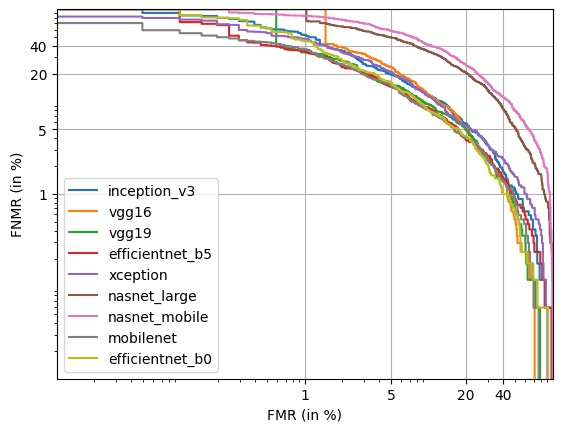
\includegraphics[width=\linewidth]{det-all.jpg}


In the following subsections each network will be inspected individually by evaluating the performance implicitly assuming a neutral FNMR and FMR rate balancing false positives and false negatives.
This allows the performance to be differentiated in terms of certain materials.



\subsection{MobileNet}
\begin{minipage}[c]{0.7\textwidth}
    Bona fide fingerprints were correctly detected with an accuracy of 89.1\%, while presentation attacks were detected correctly with 93.19\%.
    None of the materials show significant variance from each other and are within a range of 92.0\% and 94.7\%.
    Liquid Ecoflex shows the worst deception potential.

    \medskip\centering Match Rates: 
    \begin{tabular}{ r  r  r  r |}
        CMR     & CNMR          & FNMR                 & FMR    \\
        89.11\% & 93.19\%       & 6.81\%               & 10.89\% \\
    \end{tabular} \hspace{2mm} Accuracy: 91.33\%
\end{minipage}
\hfill
\begin{minipage}[c]{0.3\textwidth}
    \centering
    \begin{tabular}{ c   r }
    Live               &  89.1\% \\ \hline\hline
    Gelatine\_01       &  92.0\% \\ 
    Latex\_02          &  92.3\% \\
    Latex\_01          &  92.9\% \\
    Gelatine\_02       &  93.5\% \\
    Liquid\_Ecoflex\_01 & 93.5\% \\
    Liquid\_Ecoflex\_02 & 94.7\%
\end{tabular}









\end{minipage}



\subsection{Nasnet Mobile}
\begin{minipage}[c]{0.7\textwidth}

    With a CMR of 81.2\% Nasnet Mobile is the worst performer in the small network group.
    The presentation attack detection for the Latex datasets was with only 63\% slightly better than randomly assigned outcomes.
    A low precision in regards to the materials provide an interesting difference of over 20\% accuracy between Latex and Liquid Ecoflex.

    \medskip\centering Match Rates: 
    \begin{tabular}{ r  r  r  r |}
        CMR     & CNMR          & FNMR                 & FMR     \\
        81.22\% & 73.97\%       & 26.03\%              & 18.78\%  \\
    \end{tabular} \hspace{2mm} Accuracy: 77.27\%
\end{minipage}
\hfill
\begin{minipage}[c]{0.3\textwidth}
    \centering
    \begin{tabular}{ c   r }
    Live                &  81.2\%  \\ \hline\hline
    Latex\_02           &  63.5\%  \\
    Latex\_01           &  62.9\%  \\
    Liquid\_Ecoflex\_01 &  84.7\%  \\
    Liquid\_Ecoflex\_02 &  86.8\%  \\
    Gelatine\_02        &  75.0\%  \\
    Gelatine\_01        &  70.9\%  \\
\end{tabular}
\end{minipage}



\subsection{EfficientNet B0}
\begin{minipage}[c]{0.7\textwidth}

    The only CMR over 90\% is achieved by EfficientNet B0 which is the second best performer over all.
    Bona fide fingerprints were correctly detected with an accuracy of 92.5\%.
    
    \medskip\centering Match Rates: 
    \begin{tabular}{ r  r  r  r |}
        CMR     & CNMR          & FNMR                 & FMR     \\
        92.53\% & 88.92\%       & 11.08\%              & 6.23\%  \\
    \end{tabular} \hspace{2mm} Accuracy: 90.56\%
\end{minipage}
\hfill
\begin{minipage}[c]{0.3\textwidth}
    \centering
    \begin{tabular}{ c   r }
    Live               & 92.5\% \\ \hline\hline
    Gelatine\_02       & 85.0\% \\
    Liquid\_Ecoflex\_01& 89.7\% \\
    Latex\_01          & 88.2\% \\
    Latex\_02          & 90.0\% \\
    Liquid\_Ecoflex\_02& 90.0\% \\
    Gelatine\_01       & 90.5\% \\
\end{tabular}









\end{minipage}

\medskip
Out of the three tested neural networks MobileNet was performing the best on average thanks to it's high true negative detection rate.
The other two networks however have a better true positive rate.
\bigskip\hrule



\subsection{Xception}
\begin{minipage}[c]{0.7\textwidth}
    Presentation attack were able to be detected precicely with a max delta of 2.9\% and all accuracies are over 90\%.
    The overall performance is nothing outstanding and is in line with the median.

    \medskip\centering Match Rates: 
    \begin{tabular}{ r  r  r  r |}
        CMR       & CNMR      & FNMR     & FMR     \\
        86.64\%   & 91.47\%   & 8.53\%   & 13.36\%  \\
    \end{tabular} \hspace{2mm} Accuracy: 89.28\%
\end{minipage}
\hfill
\begin{minipage}[c]{0.3\textwidth}
    \centering
    \begin{tabular}{ c   r }
    Live                & 86.6\% \\ \hline\hline
    Liquid\_Ecoflex\_02 & 90.3\% \\
    Latex\_02           & 90.6\% \\
    Latex\_01           & 91.2\% \\
    Gelatine\_02        & 91.5\% \\
    Liquid\_Ecoflex\_01 & 92.1\% \\
    Gelatine\_01        & 93.2\%
\end{tabular}

\end{minipage}



\subsection{Inception V3}
\begin{minipage}[c]{0.7\textwidth}

    The performance is very similar to the previous network with the accuracies differing by only 0.08\%.
    Inception V3s bona fide detection is a little better, but in turn resentation attacks a bit worse in comparison.

    \medskip\centering Match Rates: 
    \begin{tabular}{ r  r  r  r |}
        CMR       & CNMR      & FNMR     & FMR     \\
        87.76\%   & 90.69\%   & 9.31\%   & 12.24\%  \\
    \end{tabular} \hspace{2mm} Accuracy: 89.36\%

\end{minipage}
\hfill
\begin{minipage}[c]{0.3\textwidth}

    \centering
    \begin{tabular}{ c   r }
    Live                & 87.8\% \\ \hline\hline
    Latex\_01           & 88.8\% \\
    Gelatine\_01        & 89.1\% \\
    Gelatine\_02        & 89.1\% \\
    Liquid\_Ecoflex\_01 & 91.5\% \\
    Latex\_02           & 92.4\% \\
    Liquid\_Ecoflex\_02 & 93.2\% \\
\end{tabular}


\end{minipage}



\subsection{EfficientNet B5}
\begin{minipage}[c]{0.7\textwidth}

    The highest correct non-match rate in the entire series is held by EfficientNet B5 with 96.03\% which is up to par with specialized solutions (cite livdet2017, p7).
    EfficientNet B5 is the best performer on average in the medium size category but the other two networks are very close in accuracy.

    \medskip\centering Match Rates: 
    \begin{tabular}{ r  r  r  r |}
        CMR       & CNMR      & FNMR     & FMR     \\
        82.70\%   & 96.03\%   & 3.97\%   & 17.30\%  \\
    \end{tabular} \hspace{2mm} Accuracy: 89.97\%

\end{minipage}
\hfill
\begin{minipage}[c]{0.3\textwidth}
    \centering
    \begin{tabular}{ c   r }
    Live                & 82.7\% \\  \hline\hline
    Gelatine\_01        & 94.7\% \\
    Latex\_01           & 95.9\% \\
    Gelatine\_02        & 96.2\% \\
    Liquid\_Ecoflex\_02 & 96.2\% \\
    Liquid\_Ecoflex\_01 & 96.5\% \\
    Latex\_02           & 96.8\% \\
\end{tabular}

\end{minipage}

Networks in the midrange size deliver as strong performance and are precise in their accuracies.
EfficientNet B5 has the second best accuracy as well as the best CNMR.

\bigskip\hrule


\subsection{NASNet Large}
\begin{minipage}[c]{0.7\textwidth}
    More than a fifth of all predictions were incorrect which makes NASNet Large not suitable to enhance the quality of fingerprint presentation attack detection mechanisms.
    With almost 18.2\% of difference between Latex and Liquid Ecoflex, the precision is the worst among all tested networks.

    \medskip\centering Match Rates: 
    \begin{tabular}{ r  r  r  r |}
        CMR       & CNMR      & FNMR     & FMR     \\
        80.11\%   & 79.41\%   & 20.59\%  & 19.89\%  \\
    \end{tabular} \hspace{2mm} Accuracy: 79.73\%
\end{minipage}
\hfill
\begin{minipage}[t]{0.3\textwidth}
    \centering
    
\begin{tabular}{ c   r }
    Live               &  80.1\% \\ \hline\hline
    Latex\_02           & 70.6\% \\
    Latex\_01           & 71.2\% \\
    Gelatine\_02        & 77.1\% \\
    Gelatine\_01        & 80.9\% \\
    Liquid\_Ecoflex\_02 & 87.9\% \\
    Liquid\_Ecoflex\_01 & 88.8\%
\end{tabular}
\end{minipage}



\subsection{VGG16}
\begin{minipage}[c]{0.7\textwidth}
    The second largest network in this test did not deliver any outstanding data.
    Accuracy and precision are certainly respectable and in the better half of all tested networks, but unremarkable considering the size and prediction latency.

    \medskip\centering Match Rates: 
    \begin{tabular}{ r  r  r  r |}
        CMR       & CNMR      & FNMR     & FMR     \\
        87.88\%   & 90.29\%   & 9.71\%   & 12.12\%  \\
    \end{tabular} \hspace{2mm} Accuracy: 89.19\%
\end{minipage}
\hfill
\begin{minipage}[c]{0.3\textwidth}
    \centering
    \begin{tabular}{ c   r }
    Live                & 87.9\% \\ \hline\hline
    Latex\_02           & 86.8\% \\    
    Liquid\_Ecoflex\_02 & 88.5\% \\
    Liquid\_Ecoflex\_01 & 89.7\% \\
    Latex\_01           & 91.5\% \\
    Gelatine\_02        & 92.4\% \\
    Gelatine\_01        & 92.9\% \\
\end{tabular}

\end{minipage}



\subsection{VGG19}
\begin{minipage}[c]{0.7\textwidth}
    The largest network provides solid non-match recognition, but cannot provice a good accuracy.
    A CNMR of almost 94\% is the second highest score comparable to algorithms which were handed in for LivDet2017.

    \medskip\centering Match Rates: 
    \begin{tabular}{ r  r  r  r |}
        CMR       & CNMR      & FNMR     & FMR     \\
        86.93\%   & 93.38\%   & 6.62\%   & 13.07\%  \\
    \end{tabular} \hspace{2mm} Accuracy: 90.45\%
\end{minipage}
\hfill
\begin{minipage}[c]{0.3\textwidth}
    \centering
    \begin{tabular}{ c   r }
    Live                & 86.9\% \\ \hline\hline
    Latex\_02           & 90.6\% \\ 
    Liquid\_Ecoflex\_01 & 92.4\% \\
    Liquid\_Ecoflex\_02 & 93.2\% \\
    Latex\_01           & 93.8\% \\
    Gelatine\_02        & 94.7\% \\
    Gelatine\_01        & 95.6\%
\end{tabular}

\end{minipage}


Especially with regards to NASNet Large, the additional size seems to provide no benefit to fingerprint presentation attack-detection mechanisms.
For NASNet Large in particular, the additional size does not provide any benefit to fingerprint presentation attack-detection mechanisms.
VGG16 and VGG18 ware both marginally better than the average network and did not deliver the expected accuracy or precision.
